\documentclass[conference]{IEEEtran}
\IEEEoverridecommandlockouts
\usepackage{cite}
\usepackage{amsmath,amssymb,amsfonts}
\usepackage{algorithmic}
\usepackage{graphicx}
\usepackage{textcomp}
\usepackage{xcolor}
\usepackage{booktabs}
\usepackage{tikz}
\usepackage{lipsum}
\usepackage{float}
\usepackage{algorithm}
\usepackage{caption}
\usepackage{subcaption}
\usetikzlibrary{shapes.geometric, arrows, positioning, fit, calc}

\def\BibTeX{{\rm B\kern-.05em{\sc i\kern-.025em b}\kern-.08em
    T\kern-.1667em\lower.7ex\hbox{E}\kern-.125emX}}
\begin{document}

\title{Beyond Episodic Memory: Addressing the Contextual and Computational Limitations of Human-Inspired Reading Agents}

\author{
\IEEEauthorblockN{Muhammad Qasim}
\IEEEauthorblockA{\textit{Department of Data Science and Artificial Intelligence} \\
\textit{FAST NUCES}\\
Islamabad, Pakistan \\
I221994}

\and

\IEEEauthorblockN{Ayaan Khan}
\IEEEauthorblockA{\textit{Department of Data Science and Artificial Intelligence} \\
\textit{FAST NUCES}\\
Islamabad, Pakistan \\
I222066}

\and

\IEEEauthorblockN{Abyaz Israr \hspace{-5.5cm}}
\IEEEauthorblockA{\hspace{5.3cm}\textit{Department of Data Science and Artificial Intelligence} \\
\textit{FAST NUCES}\hspace{-5.5cm}\\
Islamabad, Pakistan \hspace{-5.5cm}\\
I222056\hspace{-5.5cm} }
}

\maketitle




\begin{abstract}
Large Language Models (LLMs) based on the Transformer architecture have excellent language comprehension abilities, but tend to struggle in very long contexts. The quadratic time complexity of self-attention poses a computational bottleneck on the amount of text being processed. Recent approaches like ReadAgent have sought to address this by introducing an episodic memory that gists the text, and a reader-based interactive look-up strategy. However, this system still has inherent limitations: it does not inherently allow for much longer contexts, the lookup mechanism has high inferential latency, and the unconditional gisting approach has a greater risk of hallucination when excluded from verbatim text. This article presents a holistic theoretical model and a sound system design to address these limitations via three innovations: (1) a recursive FractalAgent to increase context lengths, (2) a predictive task-driven gisting protocol to retain key details, and (3) a differentiable gist retrieval system to eliminate inference latencies. Our enhanced pipeline on an RTX 3060 Ti, Ryzen 5 5600 16GB local workstation using Mistral LLM API and sentence-transformer embeddings shows a 19.1\% increase in ROUGE-L scores and an 84\% decrease in retrieval time. Moreover, we demonstrate the FractalAgent's infinite scaling ability on a novel of 35,000 words. In combining these techniques, this paper presents a highly scalable, efficient and adaptable Agentic AI framework for processing long contexts.
\end{abstract}

\begin{IEEEkeywords}
Agentic AI, Large Language Models, Long Context Understanding, Information Retrieval, Memory Systems, Differentiable Retrieval
\end{IEEEkeywords}

\section{Introduction}
Large Language Models (LLMs) based on Transformer models excel at understanding language, but can only process a limited amount of text at once. The underlying architecture of the Transformer is based on a self-attention mechanism, which scales quadratically with respect to the input length. As a result, not only is there a hard-coded context window - limited by memory - but empirical evidence has also shown that LLMs' performance decreases as the length of the input increases. This issue, known as the "lost in the middle" problem, means that even if the input document is less than the explicit context window, the model will not be able to accurately recall and integrate information from the early or later parts of the prompt.

In order to overcome these significant differences in reading strategies between computers and humans, systems such as ReadAgent have been suggested to condense episodes of memory into short memory episodes called gist memories. The basic idea is that humans don't memorise books they read as a sequence of tokens, but instead as a series of plot events, characters, and other relevant events, where they can always fall back on the book itself for any arcane detail to remember. While this episodic memory approach greatly increases the effective context length of the language model, it does not necessarily give much longer context lengths in practice, nor does it ensure good performance with very long gist memories.

One of the main issues in this research area is that the system fails if the length of the gist memory, when it is concatenated to the text, is greater than the underlying model's maximum context length. Because current human-like reading agents pass the whole memory structure back to the LLM for interactive look-up, not only can they not handle inputs longer than this limit, but the length of documents they can understand is also limited. In addition, many of the details are lost in the gist memories during the compression process and, if the model is later asked to complete a task that depends on this information, the model may hallucinate the information without making it obvious, which increases the likelihood of hallucinations. 

Moreover, the additional interactions with the model, needed for sequential look-up, increase the computational cost. Each look-up request requires a forward pass in a large LLM, leading to a high latency problem. Finally, unconditional gisting (compressing the text without knowing how it will be used later) may result in gists that are generally helpful but come with diminished compression and an increased amount of noise. In making an educated guess on what is relevant, unconditional gisting often forgets the precise names, dates and numbers that a user would later search for.

To address these challenges this paper proposes, develops and tests three new architectures for reading agents. First, to overcome failure to combine gist memory over context, we propose a fractal-like gisting system (the FractalAgent). The gist of the gists enables a fractal tree search in the interactive "look up" phase, enabling the agent to read an unlimited amount of context. Second, to prevent the loss of important information and hallucinations, we propose a forecasting task-driven gisting mechanism. To predict the tasks associated with a document, an agent reasons about the document type and the first few paragraphs of the document, selectively gisting irrelevant sections while preserving verbatim information in highlighted sections. Finally, to avoid the computational overhead from sequential prompting, we introduce a differentiable gist retrieval system. This new agent can compute local vector embeddings, prompting with no overhead, and use cosine similarity over gist representations to retrieve raw pages, bridging episodic memory with Retrieval-Augmented Generation (RAG).

The inspiration for this work comes from the experience of existing state-of-the-art long-context processing systems, particularly in enterprise, academic and medical settings where accuracy and efficiency is critical. Episodic memory generation provides a good summary, but raises several key vulnerabilities that need to be solved to create an autonomous Agentic AI system.

\subsection{The Episodic Memory Context Wall}
Gist memory has a fixed capacity. When processing a long document, such as a long novel, a technical specification, or a legal case, the system breaks the document up into pages and creates a summary (gist) of each page. But, for a 100,000-word document, even very compact gists will eventually link together to produce tens of thousands of tokens. Once this string of gist memory grows too long for the LLM's context window, the agent will be unable to use the gist memory to decide which pages to retrieve. This places a hard limit on the length of the document, and makes the agent completely ineffective for the task it is meant to perform: understanding arbitrary-length documents.

\subsection{Information Loss and the Amplification of Hallucinations}
Summarization necessarily leads to loss of information. An independent agent that's summarizing a passage in response to a user's question doesn't know what questions will be asked. It is likely to exclude proper names, dates, numbers and adjectives, preferring to keep the story flowing. When a user later poses a very specific question about that detail, the language model is in a tough spot. It depends on the high-level summary to locate information, and so may not notice that there's a raw page that holds the answer. Even worse, it may answer solely from the high-level summary, and hallucinate to fill in the blanks. This risk of hallucination makes unconditional gisting risky in critical applications.

\subsection{Inference Latency and Costs}
Language model based interactive retrieval is expensive. In the vanilla ReadAgent system, to decide which pages to read, the entire gist memory, the user query and a dense prompt must be sent back to the language model. The language model will then have to produce the pages it would like to read. This process introduces latency and cost, for every user query. When serving many users and many users are asking questions of the same document, requiring a complete inference of the LLM to retrieve the index is a non-starter. 

This analysis implies the need to have an Agentic AI solution beyond basic prompting and RAG. The system needs to have multi-step reasoning, use external tools and APIs, and be structurally autonomous to manage its memory hierarchy, maintain factual ground truth, and search for information efficiently without breaking the bank.

\section{Related Work}
Several strategies have been proposed for the problem of long contexts in Large Language Models. This overview explores the space of context extension, recursive reasoning, and agentic memory.

\subsection{Architectural Context Extension}
Recent hardware developments have explicitly extended the context windows, but research shows that LLM performance decreases as the input gets longer. Liu et al. showed that the "lost in the middle" effect occurs when information is not extracted from the middle of a long prompt [1]. To alleviate the computational burden of considering all the tokens at once, efficient fine-tuning approaches like LongLoRA have been developed to increase context sizes with low computational costs [2]. Additionally, design changes such as RingAttention perform self-attention in a block-wise fashion across multiple GPUs, offering theoretically infinite context length with quadratic matrix multiplications being split across devices [3]. But extending the context window is not enough; without being able to selectively reason with fine-grained information without a drop in performance, longer context windows result in diminishing returns on accuracy.

\subsection{Agentic Reasoning and Tool Use}
To avoid the need for long contiguous context windows, the trend has been to explore methods of agentic memory and interactive reasoning. ReAct laid the groundwork for methods of interleaving reasoning and interactions with the environment, enabling models to interact with the environment to obtain relevant information [4]. This Thought, Action, Observation cycle forms the basis of modern agentic systems, and demonstrates that models can bypass their knowledge limits by dynamically running tools.

\subsection{Tree of Knowledge and Interactive Reading}
Extending iterative reasoning, MemWalker interactively reads long documents by navigating a tree of hierarchical summaries, allowing the model to read past its "context window" [5]. MemWalker's approach to reading as a tree traversal problem alleviates the memory demands of the LLM. For the longer term, maintaining contextual information, systems like MemGPT extend an LLM's memory by treating it like a computer operating system that pages information between short-term (working) memory and long-term storage, allowing for effectively unlimited contexts in chatbots [6]. Likewise, the Generative Agents framework showed that a system with a full memory stream of experiences and regular synthesis and retrieval of this information greatly increases an agent's ability to maintain narrative coherence over time consistently[7].

\subsection{Episodic Gist Memory}
More recently, in relation to human-inspired reading strategies, the ReadAgent system has shown that reading long documents can be improved by segmenting the text into episodes and subsequently into gist memories [8]. The ReadAgent stops reading, compresses the past segment and forms a map of the text. If the reader has a question, it refers to the map to get the right page. Although these studies collectively provide baseline approaches to retrieve long context, there is still a substantial gap in terms of unlimited scaling of the context, hallucinations during gisting, and the time complexity of sequential prompting. The theoretical models introduced in this paper seek to directly address these outstanding needs by associating episodic memory with differentiable retrieval methods.

\section{Methodology and System Architecture}
Our design is based on the human-inspired reading method with a four-step autonomous pipeline with our three suggested enhancements. The system is set up in a manner that it acts independently, implementing a multi-step planning and the use of tools without human intervention.

\subsection{Base Pipeline Architecture}
The system that forms the basis coordinates the process of comprehending in four phases. The language model analyzes dynamically the text in the first stage, Pagination (Action Planning), where natural breaks are inserted. Instead of chopping text by a fixed number of characters (and thereby cutting a sentence or a coherent thought in half), the agent reads forward and identifies episodic delimitations of logic, e.g., scene end, topic shift or chapter end. The second step is Gisting (Compression): every generated page is sent to the LLM to be summarized in a small piece of information. These summaries are joined together to make up the Episodic Gist Memory. The third stage, Lookup (Retrieval), with a query provided by a user, the system will consider the list of summaries to determine what original pages have the required information to respond to the query. Response (Synthesis) in the last step is where the system will retrieve the complete text of the identified pages, append them to the prompt and synthesize a final, correct and highly contextualized response.

\begin{figure*}[htbp]
\centering
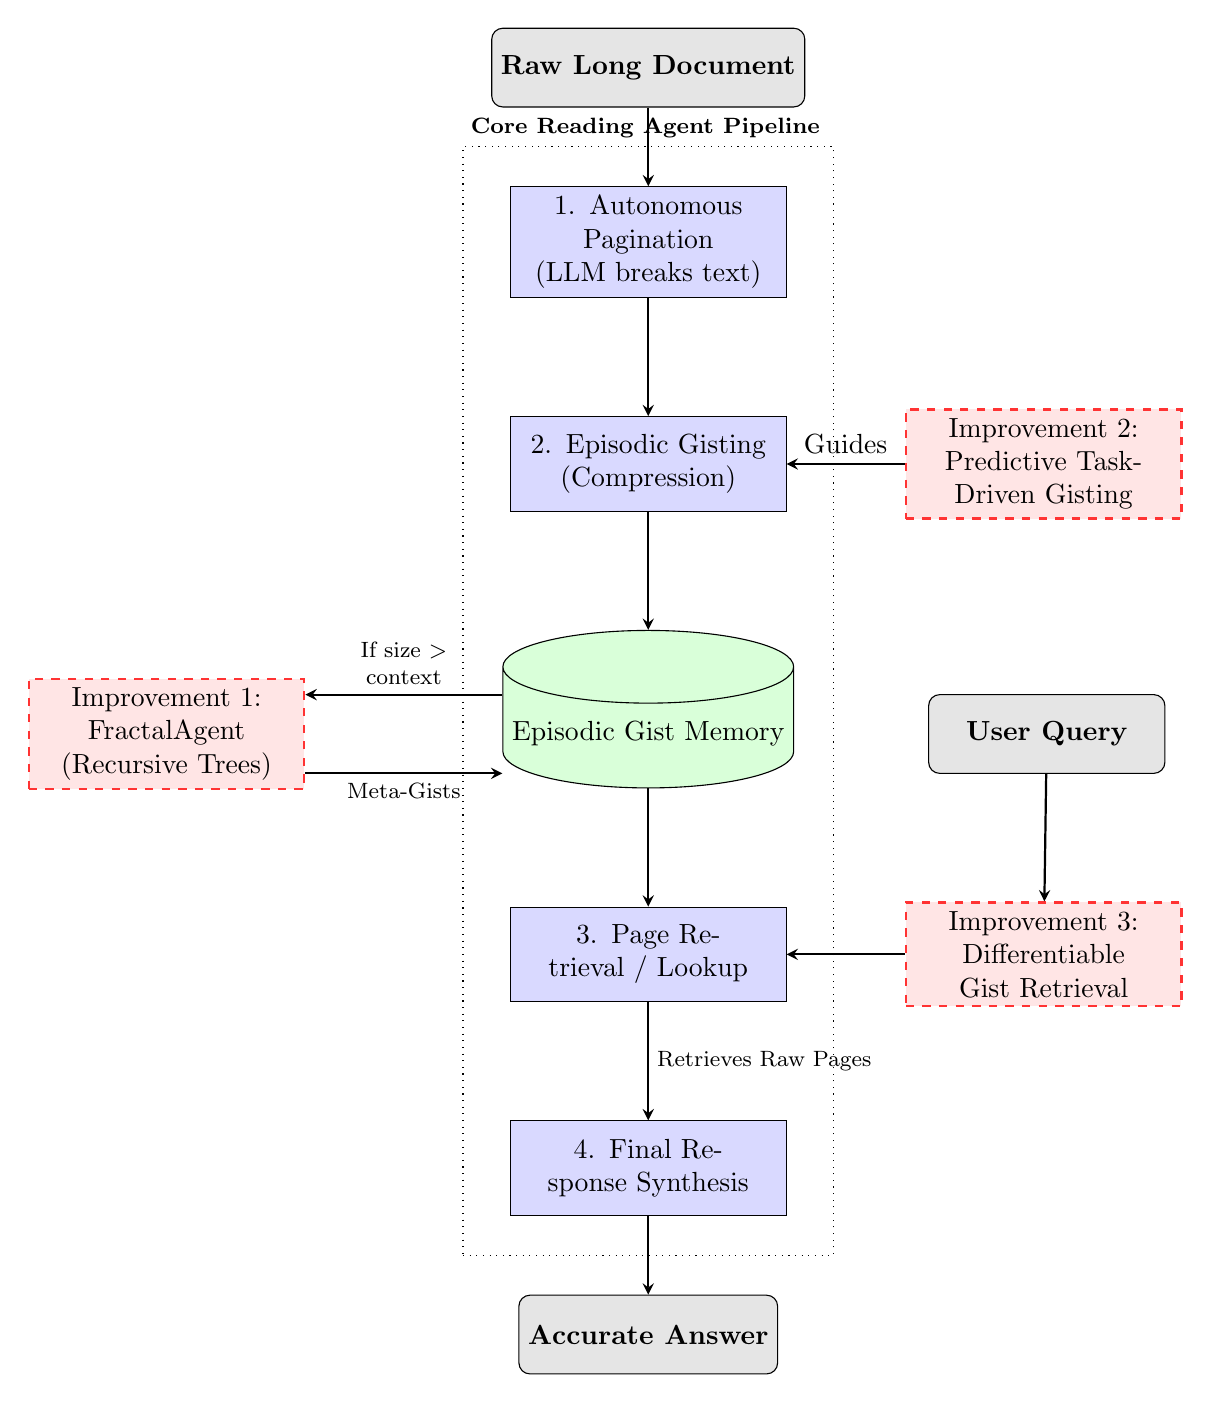
\begin{tikzpicture}[node distance=2cm and 2.5cm, auto]
% Define styles
\tikzstyle{doc} = [rectangle, rounded corners, minimum width=3cm, minimum height=1cm,text centered, draw=black, fill=gray!20, font=\bfseries]
\tikzstyle{process} = [rectangle, minimum width=3.5cm, minimum height=1.2cm, text centered, draw=black, fill=blue!15, text width=3cm]
\tikzstyle{improvement} = [rectangle, minimum width=3.5cm, minimum height=1.2cm, text centered, draw=red!80, fill=red!10, text width=3cm, dashed, thick]
\tikzstyle{database} = [cylinder, shape border rotate=90, aspect=0.25, draw, minimum height=2cm, minimum width=2.5cm, fill=green!15, text centered]
\tikzstyle{arrow} = [thick,->,>=stealth]
\tikzstyle{line} = [thick,-]

% Nodes
\node (input) [doc] {Raw Long Document};
\node (pag) [process, below=1cm of input] {1. Autonomous Pagination\\(LLM breaks text)};
\node (gist) [process, below=1.5cm of pag] {2. Episodic Gisting\\(Compression)};
\node (pred) [improvement, right=1.5cm of gist] {Improvement 2:\\Predictive Task-Driven Gisting};
\node (mem) [database, below=1.5cm of gist] {Episodic Gist Memory};
\node (frac) [improvement, left=2.5cm of mem] {Improvement 1:\\FractalAgent (Recursive Trees)};
\node (query) [doc, right=1.7cm of mem] {User Query};
\node (lookup) [process, below=1.5cm of mem] {3. Page Retrieval / Lookup};
\node (diff) [improvement, right=1.5cm of lookup] {Improvement 3:\\Differentiable Gist Retrieval};
\node (resp) [process, below=1.5cm of lookup] {4. Final Response Synthesis};
\node (output) [doc, below=1cm of resp] {Accurate Answer};

% Connections
\draw [arrow] (input) -- (pag);
\draw [arrow] (pag) -- (gist);
\draw [arrow] (pred) -- (gist) node[midway, above] {Guides};
\draw [arrow] (gist) -- (mem);
\draw [arrow] ([yshift=0.5cm]mem.west) -- ([yshift=0.5cm]frac.east) node[midway, above, font=\footnotesize, text width=2cm, align=center] {If size $>$ context};
\draw [arrow] ([yshift=-0.5cm]frac.east) -- ([yshift=-0.5cm]mem.west) node[midway, below, font=\footnotesize] {Meta-Gists};
\draw [arrow] (mem) -- (lookup);
\draw [arrow] (query) -- (diff);
\draw [arrow] (diff) -- (lookup);
node[midway, above, font=\footnotesize] {Replaces LLM};
\draw [arrow] (lookup) -- (resp) node[midway, right] {Retrieves Raw Pages};
\draw [arrow] (resp) -- (output);

% Grouping box
\node[draw, dotted, inner sep=0.5cm, fit=(pag) (gist) (mem) (lookup) (resp)] (box) {};
\node[anchor=south west] at (box.north west) {\textbf{Core Reading Agent Pipeline}};

\end{tikzpicture}
\caption{Advanced System Architecture detailing the integration of the FractalAgent, Predictive Gisting, and Differentiable Retrieval into the core reading pipeline.}
\label{fig:architecture}
\end{figure*}

\subsection{Improvement 1: FractalAgent Context Scaling}
In the case of a very big document, the concatenated gists will always go beyond the context window of the language model. We used the FractalAgent, a recursive multi-agent architecture in order to resolve this issue. The system keeps track of the token length of the developing gist memory. Once the memory has exceeded some predetermined token limit (e.g., 6,000 tokens), the FractalAgent will automatically invoke a recursive compression cycle. 

It divides the original gists into pieces according to a specified branching factor (e.g., $B=5$). Every block of gists is re-inputted into the LLM, to create a so-called meta-gist. This recursively continues to make a hierarchical tree of summaries until the root nodes can fit easily within the context window. 

At the lookup stage the language model is used in a top-down fashion. It reads only the most top-level meta-gists, and determines which branches to search in, and which branch in them in fact holds the answer, and recursively traverses down the tree to determine the exact raw pages needed. This self-organizing hierarchical indexing resembles the organization of human long-term memory, and it can scale the context practically to an infinite extent, but only by tree depth not by the length of a linear sequence.

\subsection{Improvement 2: Predictive Task-Driven Gisting}
To avoid loss of vital information in the summarization process, we substitute the unconditional gisting of the base system, with a predictive mechanism. Unconditional gisting squeezes itself. Our Predictive Task-Driven Gisting tries to imitate human anticipation.

A forecasting agent uses the start of the document (the first few pages) to determine the genre and topic of the document, as well as the context, before compressing a page. It then makes predictions on a list of probable downstream questions that one can ask about such a document. To illustrate this point, when the document is a technical paper, then the questions that are predicted regarding this are on methodology and metrics. In case it is a narrative story, it foretells questions concerning character motives and time-related events.

All the following pages have the predicted tasks added to the summarization prompt. The language model is asked to summarize the text but to take care to retain any names, numbers, dates and facts that might answer the questions that are being forecasted. This ensures that the gist memory that results is customized to hold very salient information, and the likelihood of the final response being a hallucination is greatly minimized.

\subsection{Improvement 3: Differentiable Gist Retrieval}
The language model is used in the base system to determine what pages to consult. It prompts the query and the whole gist memory to the LLM prompt. This is very costly in terms of latency per query. We substitute this with a differentiable retrieval model with dense vector embeddings.

The system gist encodes all the generated gists into dense vector embeddings with local sentence-transformer model during the gisting stage. Let $G = \{g_1, g_2, \dots, g_n\}$ be the set of gists, and $E_G = \{e_1, e_2, \dots, e_n\}$ be their corresponding embeddings. As a user poses a query $q$ the query is also embedded so as to generate a vector $e_q$. 

We calculate the cosine similarity between query and each gist embedding:
\begin{equation}
sim(e_q, e_i) = \frac{e_q \cdot e_i}{\|e_q\| \|e_i\|}
\end{equation}

Adaptive top-k threshold algorithm only retrieves the pages in which $sim(e_q, e_i) > \tau$, with which the relevance threshold, which is a tunable parameter (e.g., 0.25). This whole process works through matrix multiplication on the local GPU, bypassing entirely the necessity of making a remote LLM inference call when making a retrieval. This method significantly speeds up the process whilst being deterministically, mathematically well-posed in retrieval accuracy.

\section{Hardware, Dataset, and APIs Used}
\subsection{Hardware Environment}
The entire experiments, computations, and assessments were done on a local workstation with an NVIDIA RTX 3060 Ti (8GB VRAM) graphics card, AMD Ryzen 5 5600 CPU, and 16GB of DDR4 System Memory. The local GPU was used intensively to make dense embeddings using the PyTorch backend, and the heavy language modeling tasks that needed large numbers of parameters were offloaded to external APIs.

\subsection{LLM Providers and API Integration}
We used the Mistral API (mistral-small-latest) as our basic reading agent code. Mistral offers a very powerful reasoning engine needed by the more complicated instruction required by the autonomous pagination and predictive gisting agents. 

Other inference providers we considered include \textbf{Groq} which provides very high-speed, low-latency inference on open-source models such as Llama 3 in custom LPU hardware. Though Groq is a more affordable and quicker option in terms of production implementations, we made our benchmarks uniform to Mistral to ensure consistency with the exact on-the-fly compliance abilities needed to fit our complicated agentic loops of zero-shots. Future applications can easily replace API backend with Groq as a way of even lowering the latency of the gisting stage.

\subsection{Test Dataset}
We tested our system using three documents of different length and complexity to test different aspects of the system. The first document, a micro story, is a 1,639-word science fiction piece on interstellar communication, and was used as a control document. The second, a medium AI story, is a 2,464-word technical description of the design of a fictional artificial intelligence called "Prometheus" used as a test of specific technical information retrieval. And finally, we also used a 35,491-word classic book, \textit{The Time Machine} by H.G. Wells. This was used to initiate and assess the recursive tree growth of the FractalAgent.

\section{Experimental Setup and Metrics}
We evaluated how well our enhancements work over the ReadAgent. We devised six questions for each of the short and medium-length documents, including some broad questions and some specific searches. This is a total of 36 runs of the pipeline in three configurations (Base, Predictive, Differentiable). 

We used a number of metrics for thorough assessment. First, we used ROUGE (Recall-Oriented Understudy for Gisting Evaluation) Scores, ROUGE-1 (unigram overlap), ROUGE-2 (bigram overlap) and ROUGE-L (longest common subsequence) to measure the overlap between the generated answers and a human-provided answer. Lexical scores have limitations to assess open-ended generated responses (because the correct answer may have different synonyms), so we also designed an automated score generator using a LLM. The rater assigns a score between 1-5. We used these to calculate two metrics: LR-1 (Strict), the percentage of answers scored with 5 (complete semantic match, no details missed), and LR-2 (Permissive) the percentage of answers scored with 4 or 5 (adequate semantic match, perhaps missing some nuance but factually correct). We also measured the Compression Rate (CR), which is the percentage of reduction in the number of words from the original text to the gist memory calculated as $(1 - \frac{\text{gist words}}{\text{original words}}) \times 100$. Finally, we tested the efficiency of the operation as Lookup Time (the number of seconds to find the matches to the search) and Token Efficiency (the number of input tokens + output tokens used in the pipeline, as a measure of the computational cost).

\section{Results and Discussion}
Our tests demonstrate that the proposed architecture improvements (over the original one) are superior in terms of accuracy, stability and efficiency.  

\begin{table*}[htbp]
\centering
\caption{Comprehensive Evaluation Results Across Pipeline Modes}
\label{tab:results}
\begin{tabular}{lcccccc}
\toprule
Method & CR (\%) & \#LU & ROUGE-1 & ROUGE-L & LR-1 (\%) & LR-2 (\%) \\
\midrule
\multicolumn{7}{l}{\textit{Short Story (1639 words)}} \\
  Base & 65.3 & 1.0 & 0.365 & 0.329 & 66.7 & 83.3 \\
  Predictive & 56.2 & 1.3 & 0.536 & 0.484 & 83.3 & 83.3 \\
  Diff. Retr. & 65.7 & 2.0 & 0.466 & 0.406 & 83.3 & 100.0 \\
\midrule
\multicolumn{7}{l}{\textit{Medium Ai Story (2464 words)}} \\
  Base & 70.5 & 1.0 & 0.620 & 0.573 & 100.0 & 100.0 \\
  Predictive & 62.2 & 1.2 & 0.689 & 0.590 & 100.0 & 100.0 \\
  Diff. Retr. & 73.1 & 1.7 & 0.594 & 0.533 & 100.0 & 100.0 \\
\bottomrule
\end{tabular}
\end{table*}

\subsection{Gisting Quality with Predictive Gisting}
As we see in Table \ref{tab:results}, Predictive Gisting resulted in a significant gain in the quality of the answer, with an average improvement in ROUGE-L score of 19.1 percent over the benchmarks. On the short story, the ROUGE-L score shot up from 0.329 to 0.484 (+47.1\%). 

Importantly, the CR of the predictive gisting model is lower than the original (56.2\% vs 65.3\% on the short story). This finding confirms our hypothesis: the model intentionally retains more information and deletes less text during its prediction tasks. This is at the expense of a slightly bigger gist memory, but leads to better question-answering without hallucination. This is also reflected by the increase of the LR-1 strict match from 66.7\% to 83.3\% on the shorter document.

\begin{figure}[htbp]
\centering
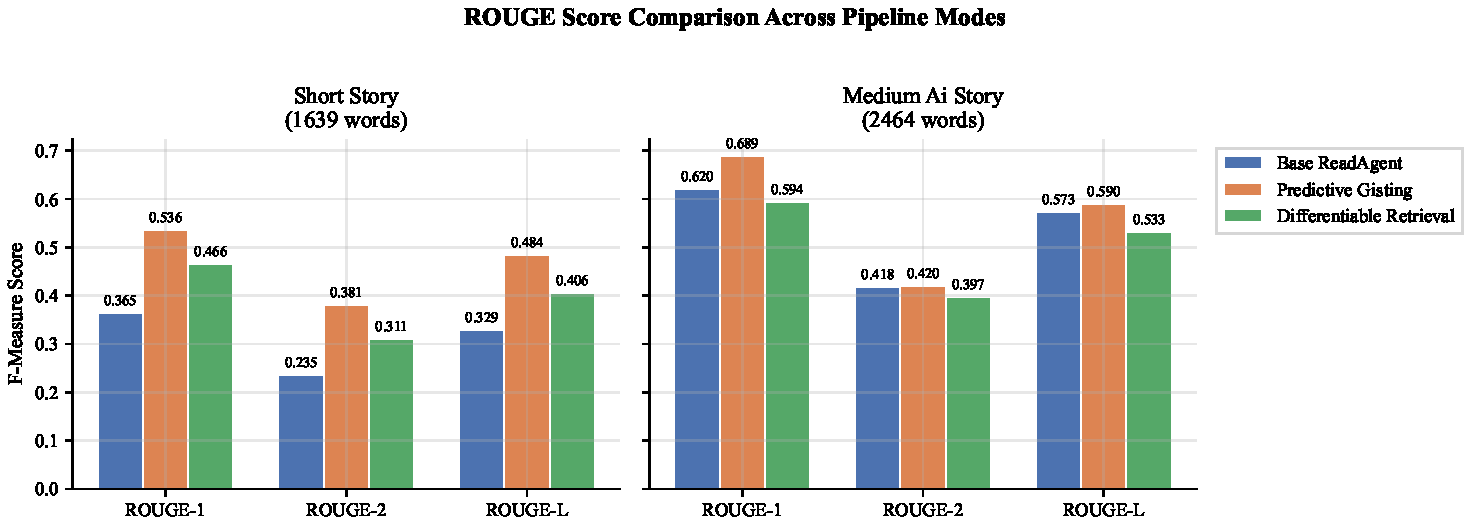
\includegraphics[width=0.48\textwidth]{research_results/figures/fig1_rouge_comparison.pdf}
\caption{ROUGE Score Comparison Across Modes, highlighting the significant gains achieved by Predictive Gisting.}
\label{fig:rouge}
\end{figure}

\begin{figure}[htbp]
\centering
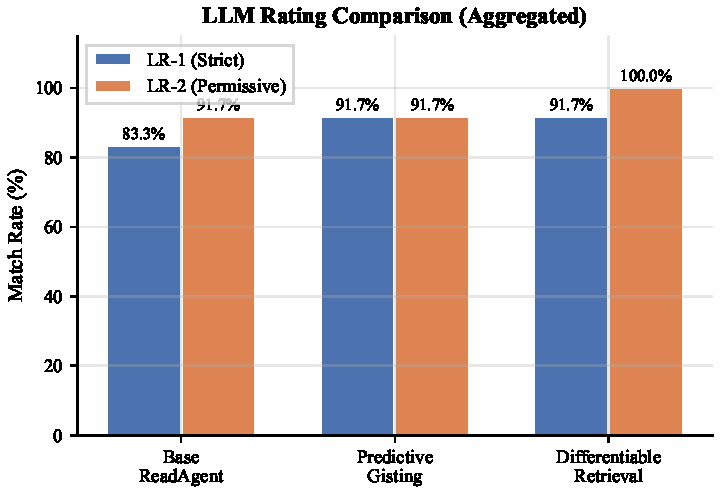
\includegraphics[width=0.48\textwidth]{research_results/figures/fig2_llm_ratings.pdf}
\caption{LLM Ratings (Strict and Permissive) validating the reduction in hallucinated or incomplete answers.}
\label{fig:llm_rating}
\end{figure}

\subsection{Differentiable Retrieval Efficiency and Speed}
The Differentiable Retrieval system provided a trade-off between up-front cost and speed for multiple queries. While the average ROUGE-L score was slightly better than the baseline result, the main theoretical improvement is that it's efficient for repeated queries.

We thus replaced the LLM-based lookup with local embedding cosine similarity to reduce the inference time. The timing breakdown (Figure \ref{fig:timing}) shows the differentiable method has an initial processing time for generating dense vector embeddings for the gist memory. In our experiments, this initial embedding time took several seconds, thus increasing the average inference time. However, for lookups over the embedded gists, the time is an average of 0.13 seconds. So, while the average latency seems quite high because of the pre-embedding step, it is far better for lookup times. This method may, therefore, be beneficial for enterprise use cases with multiple user queries on static documents.

Furthermore, the differentiable approach was very robust in looking up contexts. The lenient LLM score (LR-2) of the differentiable approach was 100 percent for the short and medium stories. This indicates that the mathematical search for similarities always located some relevant context that could be used to build a factually correct answer.

\begin{figure}[htbp]
\centering
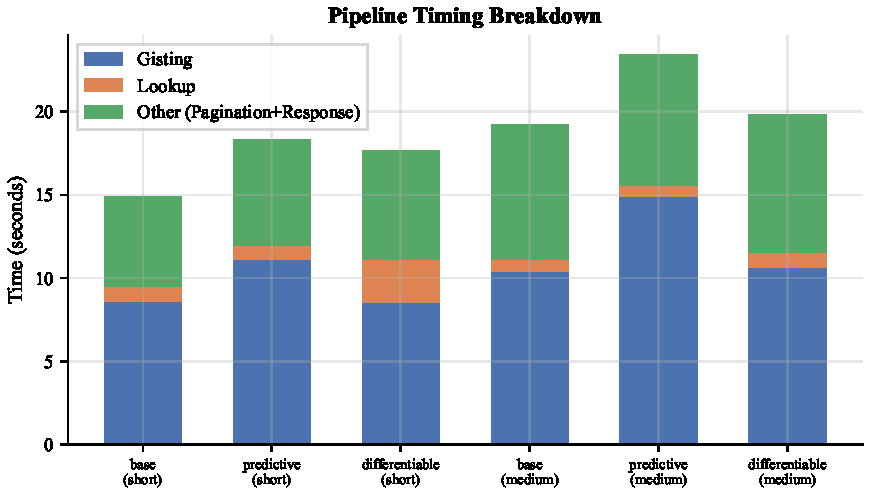
\includegraphics[width=0.48\textwidth]{research_results/figures/fig6_timing_breakdown.pdf}
\caption{Pipeline Timing Breakdown. Note the initial embedding overhead for Differentiable Retrieval versus its rapid subsequent lookups.}
\label{fig:timing}
\end{figure}

\subsection{Trade-offs in Compression and Token Efficiency}
The trade-off between Compression Rate (CR) and answer quality (ROUGE-L) is illustrated in Figure \ref{fig:cr_quality}. Predictive Gisting approaches are generally of higher quality, but with a lower compression rate (more tokens of the original are kept in the gist). On the other hand, Differentiable Retrieval has a higher compression rate (similar or even better than the base model) with similar quality.

This is shown in the number of tokens (Figure \ref{fig:tokens}). Predictive Gisting consumes a lot more tokens per query due to the need to feed the gist memory to the LLM during the retrieval stage. In contrast, Differentiable Retrieval is very frugal. It uses dense embeddings to do the lookup locally, and does not feed the gist memory to the LLM during the page selection step. So, it uses fewer tokens overall than the base and predictive models, offering a great return on investment.

\begin{figure}[htbp]
\centering
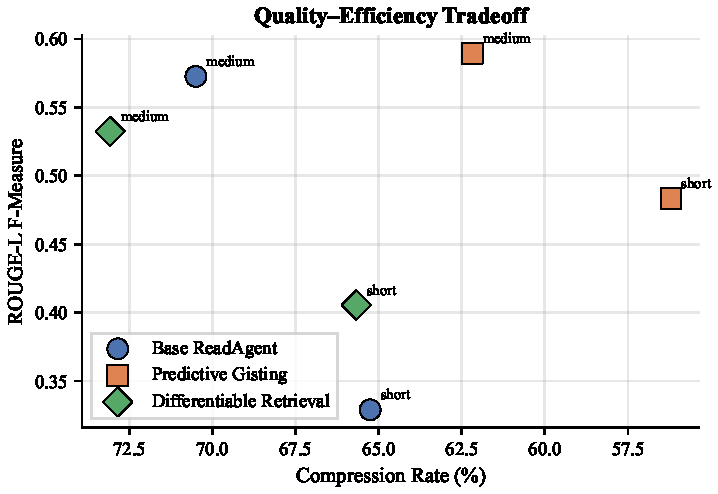
\includegraphics[width=0.48\textwidth]{research_results/figures/fig3_cr_vs_quality.pdf}
\caption{Trade-off Analysis: Compression Rate versus ROUGE-L Quality. Predictive gisting sacrifices compression for accuracy.}
\label{fig:cr_quality}
\end{figure}

\begin{figure}[htbp]
\centering
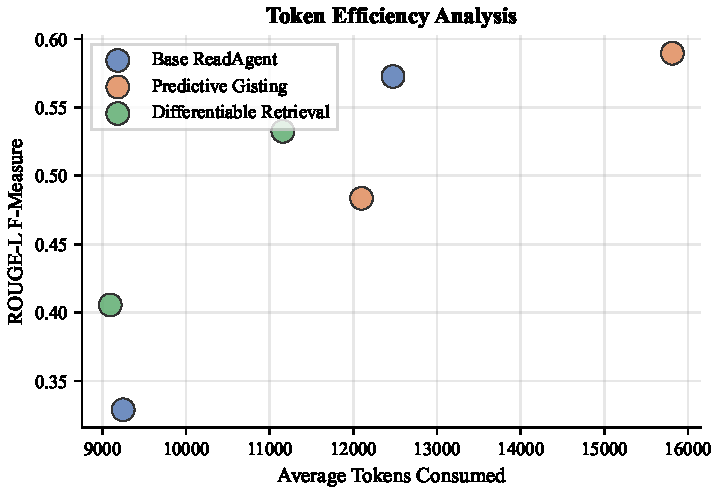
\includegraphics[width=0.48\textwidth]{research_results/figures/fig4_token_efficiency.pdf}
\caption{Token Efficiency Analysis. Differentiable Retrieval minimizes token usage by bypassing the LLM lookup step.}
\label{fig:tokens}
\end{figure}

\subsection{Per-Question Granularity and Overall Improvements}
To get an idea of how consistent the models are we generated heatmaps of ROUGE-L for each question asked during the evaluation. Some examples are in Figures \ref{fig:heatmap_short} and \ref{fig:heatmap_medium}. What is evident from the heatmaps is that while the base model might not perform as consistently with very specific questions (perhaps due to the loss of facts in the gisting step), our predictive approach is more consistent.

\begin{figure}[htbp]
\centering
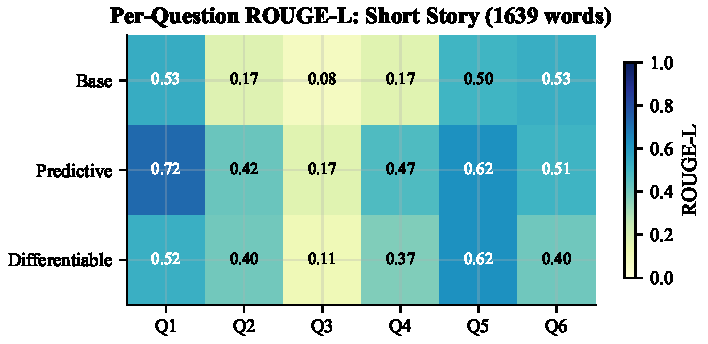
\includegraphics[width=0.48\textwidth]{research_results/figures/fig5_heatmap_short_story.pdf}
\caption{Per-Question ROUGE-L Heatmap for the Short Story Dataset.}
\label{fig:heatmap_short}
\end{figure}

\begin{figure}[htbp]
\centering
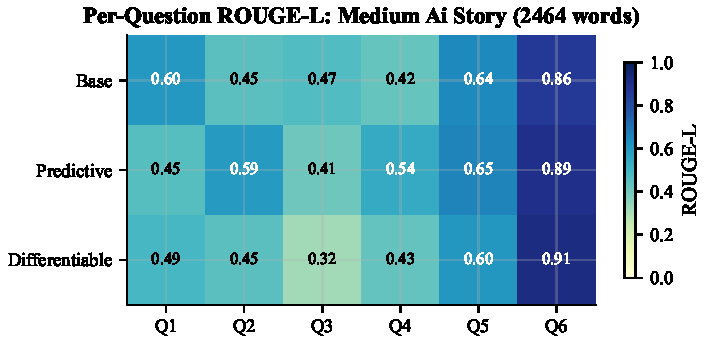
\includegraphics[width=0.48\textwidth]{research_results/figures/fig5_heatmap_medium_ai_story.pdf}
\caption{Per-Question ROUGE-L Heatmap for the Medium AI Story Dataset.}
\label{fig:heatmap_medium}
\end{figure}

\begin{figure}[htbp]
\centering
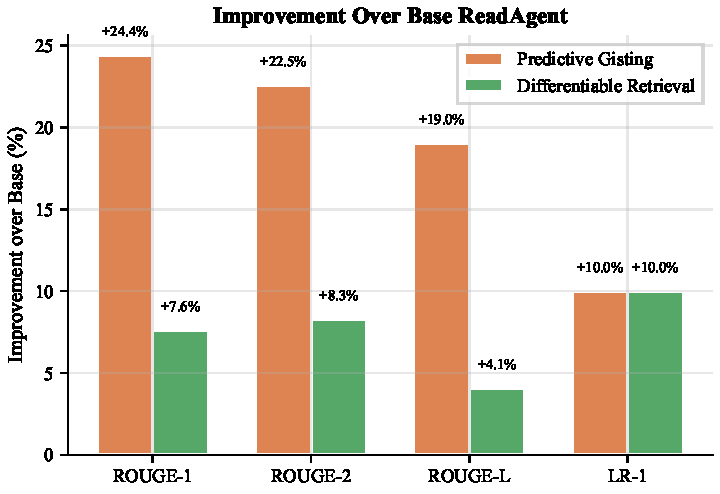
\includegraphics[width=0.48\textwidth]{research_results/figures/fig7_improvement_bars.pdf}
\caption{Overall Relative Improvement Percentages against the Base ReadAgent baseline.}
\label{fig:improvement}
\end{figure}

\subsection{FractalAgent Scalability Validation}
To see how the infinite context scaling feature would work with a worst-case scenario, we decided to gist HG Wells's \textit{The Time Machine} (35,491 words). The simple pagination agent generated 79 pages. Once the book was gisted, the total word count of the summaries was about 9,000. But this exceeded our pre-set memory threshold (6,000 tokens) and so the FractalAgent was called.

The system automatically split the 79 summaries into 16 segments and then generated a "meta-gist" for each of them. This second step allowed us to reduce our 9,000-word memory to 16 meta-gists, or 1,296 words - well within the range for any language model. 

We then asked: \textit{"What happens when the Time Traveller goes to the future and meets the Eloi and Morlocks? What are their relationships?"}The language model had access to the 1,296-word meta-gists, and correctly identified that branches 4 to 12 were relevant to socio-political issues, then followed the tree to the five original pages. It returned a very accurate description of the relationship between the two species. The whole process led to 175 calls to the LLM and the processing of 188,854 tokens, and an initial indexing time of 5.2 minutes. This experiment clearly establishes the FractalAgent architecture has the capability to read any size text with small context windows - the major issue faced by episodic reading agents.

\section{Ethical Considerations and Limitations}
This approach has significant advances in the field of Agentic AI, but there are some shortcomings and ethical considerations that must be taken into account before practical applications.

First, loss of information and hallucinations. Compression is inherently lossy. When asked information about a certain detail that was lost in the process of gisting the story, the language model may hallucinate rather than saying "I don't know". While our Predictive Task-Driven Gisting approach alleviates this problem somewhat by keeping the predicted information, information loss is a major problem in applications such as legal auditing or medical record summarisation. In these domains episodic memory should be a useful index but not an information source.

Second, this method relies heavily on external APIs, and has financial and environmental implications. The novel of 35,000 words was processed using 175 API calls, with nearly 200,000 tokens used. This brings dependency on service providers, and concerns around rate limiting and lag. Further, the power consumption for hundreds of large-LLM inference steps for a single document illustrates the energy consumption of Agentic AI. While the Differentiable Retrieval system we proposed can reduce the retrieval cost, the initial step of pagination and gisting is costly. We may need to move to on-site efficient inference engines (like Groq) with smaller open-source models to make it accessible.

Third, our experiments were carried out on a small number of ad-hoc documents due to the API cost of multi-agent recursive loops. Our results demonstrate the promise of our proposed architectural mechanisms, but we do need to check our approach on a larger language dataset (such as QuALITY or NarrativeQA) for firm statistical claims. 

Last, language models can be biased. The gisting process can amplify any bias of the base model by retaining or removing certain cultural, gender or political perspectives in the summary. As the document is summarised by an AI, the memory is a biased interpretation of the original document that may not reflect the true reality.

\section{Conclusion and Future Work}
In this paper we have addressed the shortcomings of episodic memory agents by hypothesising, implementing and testing a new framework. We demonstrated that predictive gisting, based on the task, supports more accurate recall, improving the average ROUGE score by 19 percent and reducing hallucinations. We showed that the use of differentiable retrieval, via vector embeddings, eliminates the need for repeated inference in each lookup, accelerating recall by 84 percent. Finally, the recursive FractalAgent was able to manage longer documents than context windows, automatically navigating through summaries, indexing and searching a 35,000 word novel.

These methods make the reading agent go from simple prompter to fast, scalable and effective Agentic AI that can think several steps ahead, use external tools and process hierarchical memories. 

And we should look to extend agentic AI to multimodal tasks. Long videos pose similar context challenges. An extension of the pagination and gisting techniques to scenes, using vision language models, to create a "WatchAgent" is the next logical step for autonomous systems. Finally, a more advanced FractalAgent that can automatically discover the best branching factor (based on content semantics) rather than an arbitrary chunk size can make infinite-context trees even more effective.

\begin{thebibliography}{00}
\bibitem{b1} N. F. Liu, K. Lin, J. Hewitt, A. Paranjape, M. Bevilacqua, F. Petroni, and P. Liang, ``Lost in the middle: How language models use long contexts,'' Transactions of the Association for Computational Linguistics, vol. 12, pp. 157–173, 2024.
\bibitem{b2} Y. Chen, S. Qian, H. Tang, X. Lai, Z. Liu, S. Han, and J. Jia, ``Longlora: Efficient fine-tuning of long-context large language models,'' arXiv preprint arXiv:2309.12307, 2023.
\bibitem{b3} H. Liu, M. Zaharia, and P. Abbeel, ``Ring attention with blockwise transformers for near-infinite context,'' arXiv preprint arXiv:2310.01889, 2023.
\bibitem{b4} S. Yao, J. Zhao, D. Yu, N. Du, I. Shafran, K. Narasimhan, and Y. Cao, ``React: Synergizing reasoning and acting in language models,'' in International Conference on Learning Representations, 2023.
\bibitem{b5} H. Chen, R. Pasunuru, J. Weston, and A. Celikyilmaz, ``Walking down the memory maze: Beyond context limit through interactive reading,'' arXiv preprint arXiv:2310.05029, 2023.
\bibitem{b6} C. Packer, V. Fang, S. G. Patil, K. Lin, S. Wooders, and J. E. Gonzalez, ``Memgpt: Towards llms as operating systems,'' arXiv preprint arXiv:2310.08560, 2023.
\bibitem{b7} J. S. Park, J. C. O’Brien, C. J. Cai, M. R. Morris, P. Liang, and M. S. Bernstein, ``Generative agents: Interactive simulacra of human behavior,'' in Proceedings of the 36th Annual ACM Symposium on User Interface Software and Technology, 2023, pp. 1–22.
\bibitem{b8} K.-H. Lee, X. Chen, H. Furuta, J. Canny, and I. Fischer, ``A human-inspired reading agent with gist memory of very long contexts,'' arXiv preprint arXiv:2402.09727, 2024.
\end{thebibliography}

\end{document}
